%!TEX root = Slic3r-Manual.tex

\subsection{\texttt{SVG Output}} % (fold)
\label{sec:svg_output}
\index{SVG}
\index{DLP resin printer}
\index{powder-bed printer}

Slic3r can produce output for other types of 3D printers which require each layer to be represented as image, for example DLP resin or powder-bed printers.  These expect an image usually consisting of a white silhouette on a black background (See fig \ref{fig:example_svg_slice}).  Almost all image formats can be used (bmp, png, etc.), however, because the image may have to be scaled, it is usually desirable to use a vector format, rather than a bitmap format.  For this reason it is common to use Scalable Vector Graphics (SVG) format.

\begin{figure}[H]
\centering
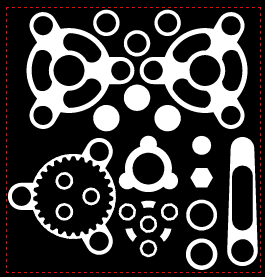
\includegraphics[keepaspectratio=true,width=0.5\textwidth]{advanced/svg_output/example_svg_slice.png}
\caption{Example SVG slice.}
\label{fig:example_svg_slice}
\end{figure}

\index{Menu!Slice to SVG...}

Slic3r provides the ability to produce SVG output suitable for such printers.  Instead of using the \texttt{Plater}, the process begins by selecting the \texttt{Slice to SVG...} option from the \texttt{File} menu.  This prompts for the source file (STL, OBJ or AMF), and when selected will prompt for where the output SVG file should be saved.  Slic3r will then go and produce the SVG file.

Attempting to view the SVG file in a browser will result in only the first layer being shown, and only the negative islands within the model (as the browser background is usually white).

\begin{figure}[H]
\centering
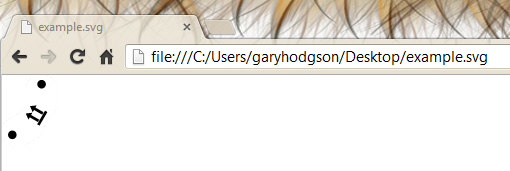
\includegraphics[keepaspectratio=true,width=0.75\textwidth]{advanced/svg_output/svg_direct_browser.png}
\caption{SVG in the browser.}
\label{fig:svg_direct_browser}
\end{figure}

For this reason a small web application was written to allow each slice to be displayed, and for it to be shown on a black background\footnote{\	exttt{http://garyhodgson.github.io/slic3rsvgviewer}}.  Navigate to the application and drag and drop the SVG file onto the screen to have it load and display.

\begin{figure}[H]
\centering
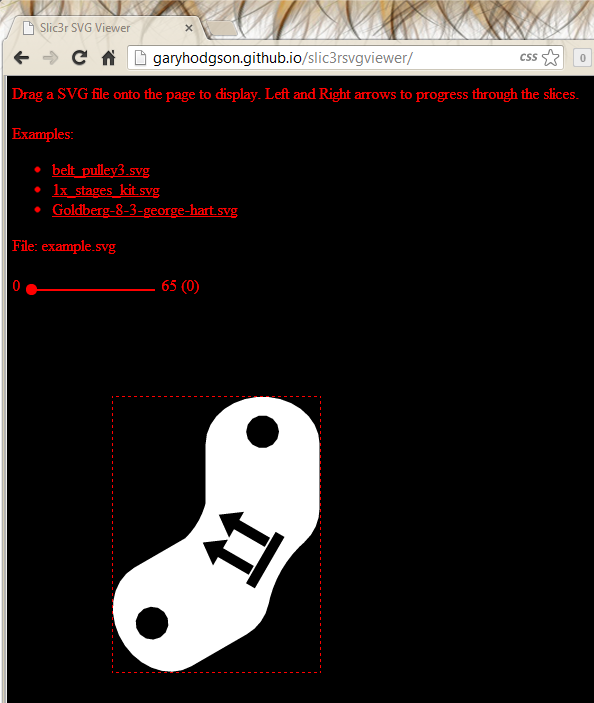
\includegraphics[keepaspectratio=true,width=0.75\textwidth]{advanced/svg_output/svg_slic3rsvg_viewer.png}
\caption{Slic3r SVG Viewer.}
\label{fig:svg_slic3rsvg_viewer}
\end{figure}

\subsubsection{\texttt{SVG Settings}} % (fold)
\label{sub:svg_settings}

The majority of options in Slic3r are not required when generating SVG, however the \texttt{Layer height} setting will dictate the number of layers.  Note that Slic3r restricts the layer height to be smaller than the nozzle diameter, so this may also have to increased if higher layers are desired.

% subsubsection svg_settings (end)

\subsubsection{\texttt{Printing with SVG}} % (fold)
\label{sub:printing_with_svg}

Whilst SVG output can be used in a range of printers, the following example shows how the file can be used with a DLP resin printer.  Using a modified version of Kliment's Printrun\footnote{\	exttt{http://garyhodgson.com/reprap/projectlayer}} the SVG file can be loaded directly and sent to a DLP projector.  The Z axis is controlled via G-Code commands sent through the printcore component, which means that standard RepRap electronics, such as RAMPS, can be used.


\begin{figure}[H]
\centering
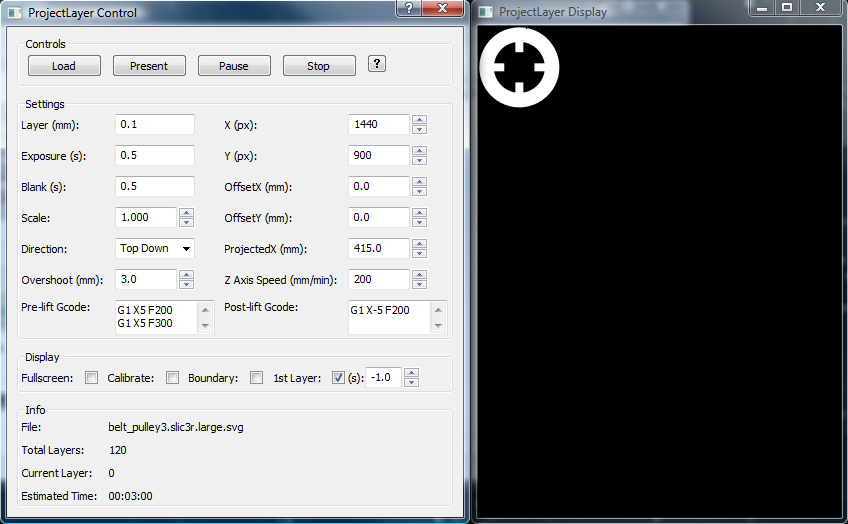
\includegraphics[keepaspectratio=true,width=0.75\textwidth]{advanced/svg_output/projectlayer.png}
\caption{Printing SVG with Projectlayer.}
\label{fig:projectlayer}
\end{figure}


% subsubsection printing_with_svg (end)

% subsection svg_output (end)
